\documentclass[12pt,a4paper]{article}
\usepackage[utf8]{inputenc} % para poder usar tildes en archivos UTF-8
\usepackage[spanish]{babel} % para que comandos como \today den el resultado en castellano
\usepackage{a4wide} % márgenes un poco más anchos que lo usual
\usepackage[conEntregas]{caratula}
\usepackage[dvipsnames]{xcolor}
\usepackage{hyperref}
\usepackage{ulem}
\usepackage{comment}
\usepackage{changepage}
\usepackage{amsmath}
\usepackage{amssymb} 
\usepackage{mathtools}
\usepackage{graphicx}
\usepackage{float}
\usepackage{caption}
\usepackage{subcaption}

\graphicspath{{images}}

\usepackage{titlesec}

% Esto fuerza el formato: Grande, Negrita, y fuente Normal
\titleformat{\section}
  {\normalfont\fontsize{16}{19}\bfseries}{\thesection}{1em}{}

% Esto ajusta el espacio para que se note más la separación
\titlespacing*{\section}{0pt}{3.5ex plus 1ex minus .2ex}{2.3ex plus .2ex}

\begin{document}

\titulo{Informe Trabajo Práctico 02}
\subtitulo{Subtítulo del tp}

\materia{Laboratorio de Datos}
\grupo{Grupo NAN}

\integrante{Rozas Chavez, Antuanette Carolina}{571/23}{antuanetterozas@gmail.com}
\integrante{Madril, Joaquin Leandro}{109/25}{madriljoaquin@gmail.com}
\integrante{Fernández Fazio, Adrián Patricio}{938/24}{adrianfernandezfazio@gmail.com}

\maketitle
\section*{Introducción}

\section*{Análisis Exploratorio}
Realizado el análisis consideramos que los atributos relevantes son los que están más al 'centro' del
cuadro en dónde empiezan a aparecer los pixeles de color negro. Observando la figura 1 pensamos que 
podemos descartar los atributos de las primeras 2 o 3 filas/columnas.

\begin{figure}[H]
     \centering
     \begin{subfigure}[b]{0.8\textwidth}
         \centering
         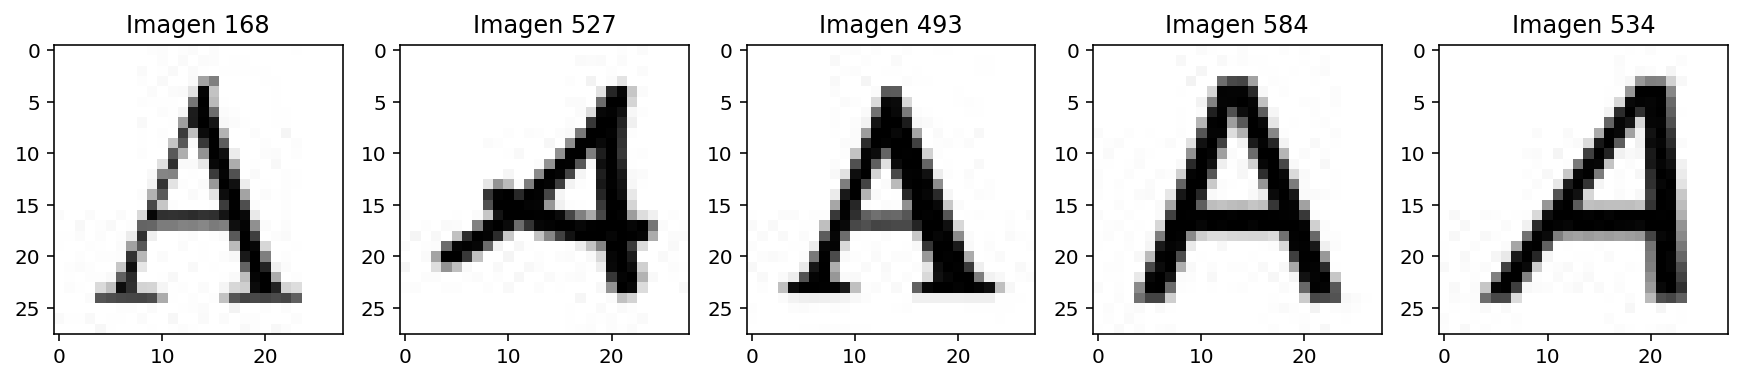
\includegraphics[width=\textwidth]{letrasA.png}
         \caption{Algunas variantes de la letra A}
     \end{subfigure}
     \hfill
     \begin{subfigure}[b]{0.8\textwidth}
         \centering
         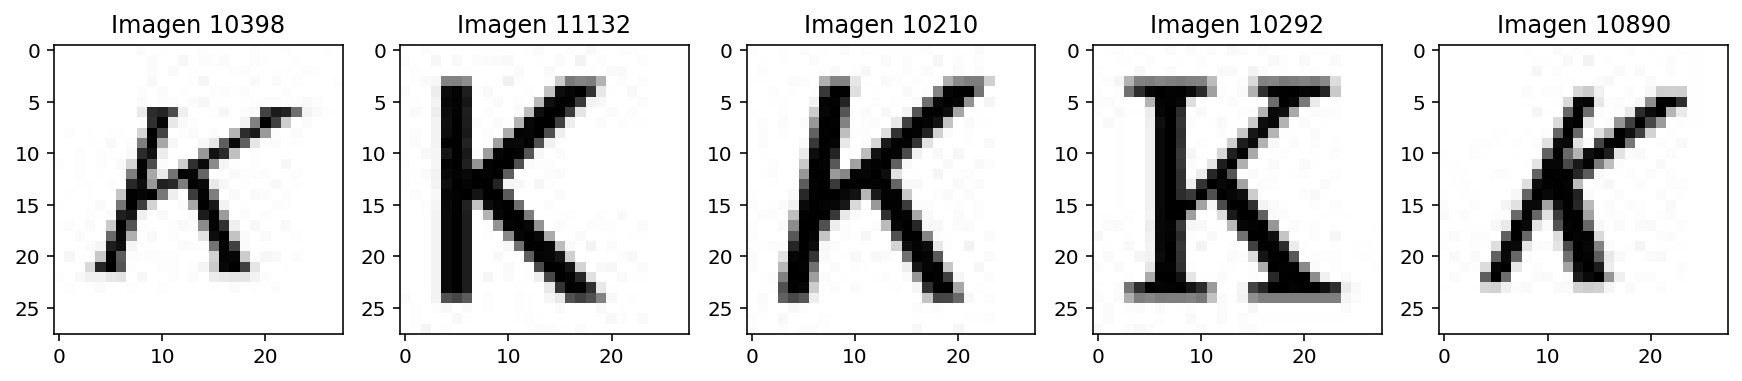
\includegraphics[width=\textwidth]{letrasK.png}
         \caption{Algunas variantes de la letra K}
     \end{subfigure}
     \hfill
     \begin{subfigure}[b]{0.8\textwidth}
         \centering
         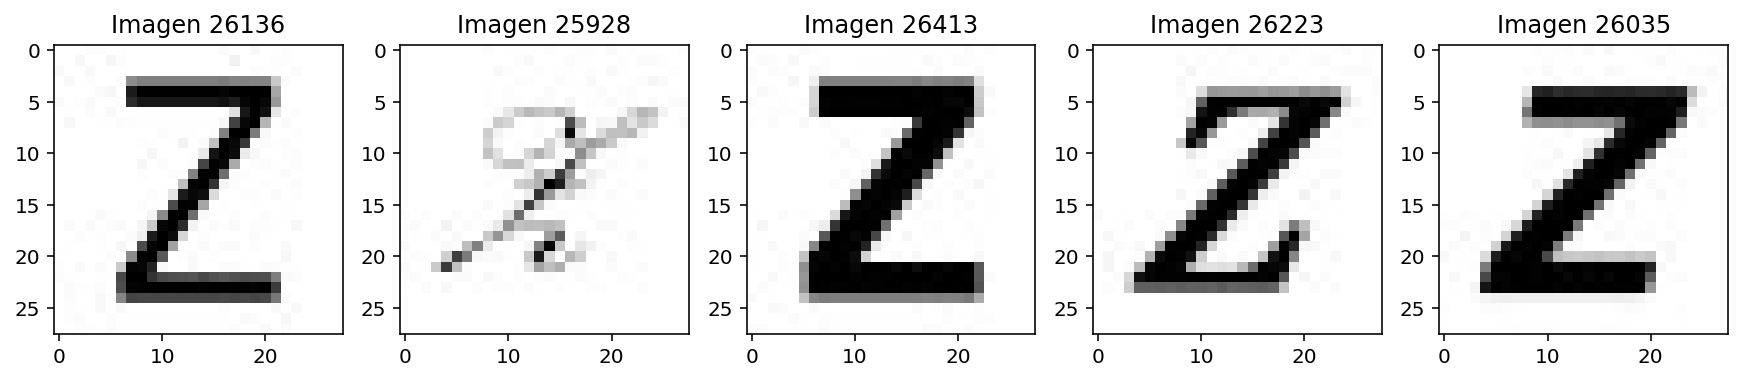
\includegraphics[width=\textwidth]{letrasZ.png}
         \caption{Algunas variantes de la letra Z}
     \end{subfigure}
     \caption{Letras A, K y Z con sus respectivas variantes}
     \label{fig:tres_graficos}
\end{figure}

\section*{Experimentos realizados}

\section*{Conclusión}
\end{document}

